\chapter{Regulacja rozmyta}
Tytułowy typ regulacji zrywa ze standardową procedurą podejmowania decyzji w sposób binarny, tzn. $1 / 0$ \cite{40}. Na Rys. \ref{crisp} przedstawiono standardową funkcję przynależności do zbioru, którą można opisać wzorem:

\begin{equation}
\mu_C = \begin{cases}
1, \quad x \in [a, b] \\
0, \quad x \notin [a, b]
\end{cases}
\end{equation}

\begin{figure}[h!]
\centering
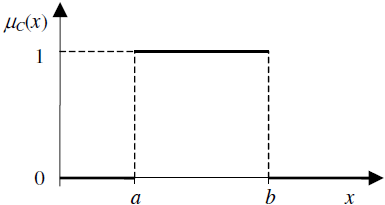
\includegraphics[width=0.5\textwidth]{pictures/crisp}
\caption{Funkcja przynależności zbioru ostrego.}
\label{crisp}
\end{figure}

Natomiast istota wnioskowania rozmytego polega na zgromadzeniu wiedzy eksperckiej, operatora procesu, wspartej odpowiedzią skokową obiektu, które pozwolą na sformułowanie zbiorów rozmytych (Rys. \ref{fuzzy_set}) oraz bazy reguł definiującej regulator rozmyty \cite{160, 170}. Funkcja przynależności zbioru rozmytego została zaprezentowana na Rys. \ref{fuzzy} i w tym przypadku dana jest wzorem:

\begin{equation}
\mu_C = \begin{cases}
0,& \quad x \leq c \vee x \geq f \\
\frac{x-c}{d-c},& \quad c \leq x \leq d \\ 
1,& \quad d \leq x \leq e \\
\frac{f-x}{f-e},& \quad e \leq x \leq f
\end{cases}
\end{equation}

\begin{figure}[h!]
\centering
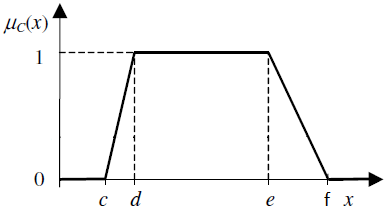
\includegraphics[width=0.5\textwidth]{pictures/fuzzy}
\caption{Funkcja przynależności zbioru rozmytego.}
\label{fuzzy}
\end{figure}

\newpage

\noindent Zmienne z odcinków $[c,d]$ oraz $[e,f]$ przyjmują wartości z przedziału $[0,1]$, w tym sensie granice zbioru przynależności są rozmyte. Natomiast wartość funkcji przynależności do zbioru określana jest stopniem przynależności. Należy w tym miejscu zwrócić uwagę na kształty funkcji przynależności. Funkcje trapezowe bądź trójkątne proste w swym zapisie, nie są różniczkowalne. Aspekt ten jest o tyle istotny, że zapewnia stabilność, zwiększa dokładność w systemach sterowania rozmytego, a także jest niezbędny podczas uczenia maszynowego, wykorzystującego metody gradientowe. Dlatego w wielu zastosowaniach przyjęło się korzystanie z innych kształtów funkcji przynależności, zapewniających różniczkowalność, takich jak: gaussowskie, dzwonowe, sigmoidalne.

\begin{figure}[h!]
\centering
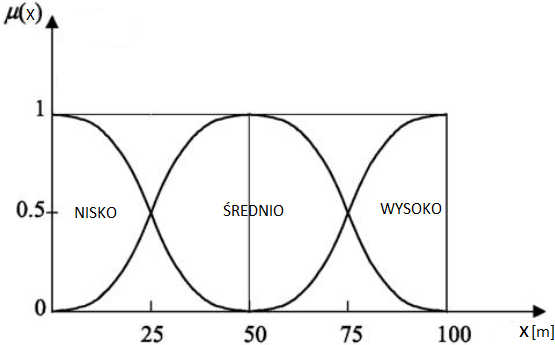
\includegraphics[width=0.75\textwidth]{pictures/fuzzy_set}
\caption{Przykładowe zbiory rozmyte.}
\label{fuzzy_set}
\end{figure}

Ważną kwestią w rozumieniu systemów rozmytych, jest pośrednik między zmienną numeryczną, a zmienną symboliczną - zmienna lingwistyczna. Na Rys. \ref{fuzzy_set} przedstawiono rozmycie zmiennej "wysokość", która przyjmuje trzy wartości: "nisko", "średnio", "wysoko" i tak można zauważyć, że wartość numeryczna $75m$ ze stopniem przynależności $0,5$ należy do zbiorów "średnio" oraz "wysoko" \cite{90, 120, 130}. \\
Po rozmyciu zmiennej lingwistycznej, określeniu stopni przynależności danych wartości do poszczególnych zbiorów pozostaje jeszcze zdefiniowanie bazy wiedzy, czyli tzw. zbioru reguł. Każda reguła składa się z części warunkowej, zwanej poprzednikiem oraz konsekwencji, określanej następnikiem. Ogólna struktura reguły w rozumieniu systemów rozmytych przyjmuje postać:

\begin{equation}
\text{JEŚLI } <poprzednik> \text{ TO } <następnik> 
\end{equation}

Poprzedniki reguł w najprostszym przypadku mogą zawierać pojedynczy warunek w innej sytuacji mogą składać się z kilku prostych warunków połączonych operacjami logicznymi (i, lub, nie).

\begin{itemize}
\item[•] warunek prosty: $\text{JEŚLI } x \text{ jest } A \text{ TO } <następnik>$ \\
\item[•] warunek złożony: $\text{JEŚLI } x_1 \text{ jest } A_1 \text{ lub } x_2 \text{ jest } A_2 \text{ i } x_3 \text{ nie jest } A_3 \text{ TO } <następnik>$ \\
\end{itemize}

\newpage

W przypadku następników reguł wyróżnić można ich trzy postaci:

\begin{enumerate}
\item Następnik ostry
\begin{equation}
\text{JEŚLI } <poprzednik> \text{ TO } y = y_a
\end{equation}

\item Następnik rozmyty 
\begin{equation}
\text{JEŚLI } <poprzednik> \text{ TO } y \text{ jest } Y_a
\end{equation}

\item Następnik funkcyjny
\begin{equation}
\text{JEŚLI } <poprzednik> \text{ TO } y = f(x_1, x_2, ... , x_k)
\end{equation}
\end{enumerate}

\noindent Szczególnie istotne oraz wykorzystywane w praktyce są dwie ostatnie wymienione metody. Następniki w postaci zbiorów rozmytych są z powodzeniem wykorzystywane w modelach Mamdaniego \cite{170, 90}, gdzie wykorzystując wiedzę eksperta można z dużą dokładnością sterować obiektem regulacji w sposób rozmyty. Częstą praktyką w tym podejściu jest budowanie tablicy decyzyjnej, która w stosunkowo prosty i przejrzysty sposób redukuję bazę reguł do tabeli \cite{170}. \\
W kontekście niniejszej pracy skupiono się przede wszystkim na następnikach funkcyjnych opisujących modele Takagi - Sugeno, którym poświęcono następny rozdział. 

\section{Modele Takagi-Sugeno}
Projektowanie modeli Takagi-Sugeno składa się z następujących etapów:

\begin{enumerate}
\item Obliczenie poziomów aktywacji reguł
\item Wyznaczenie konkluzji - obliczenie wartości następników funkcyjnych poszczególnych reguł
\item Wyznaczenie konkluzji końcowej - zsumowanie wartości następników funkcyjnych - ważone i normowane - z uwzględnieniem sił odpalenia reguł, co opisuje wzór \ref{wniosek}.
\end{enumerate}

\begin{equation}
y = \frac{\sum_{j=1}^r w^j y^j}{\sum_{j=1}^r w^j}
\label{wniosek}
\end{equation}

\noindent gdzie:
\begin{itemize}
\item[•] $r$ - liczba reguł
\item[•] $w^j$ - siły odpalenia poszczególnych reguł
\item[•] $y^j$ - wartości odpowiednich następników funkcyjnych
\end{itemize}

Ogólnie modele rozmyte służą do aproksymacji funkcji nieliniowych stąd w przypadku modeli Takagi-Sugeno następniki funkcyjne występują najczęściej w postaci funkcji wielomianowych pierwszego rzędu \cite{160, 170}:

\begin{equation}
\text{JEŚLI } <poprzednik> \text{ TO } y = a_0 + \sum_{j=1}^n a_jx_j
\end{equation} 

Natomiast w pracy skupiono się jakie korzyści może przynieść zastosowanie nieliniowych - hiperbolicznych - następników. Według autorów \cite{80} pozwala to na zmniejszenie liczby zbiorów rozmytych, a tym samym reguł.

\newpage

\section{Podejście PDC}
Podejście PDC (\textit{Parallel Distributed Combensation}) zakłada dedukcję regulatora za pomocą modelu Takagi-Sugeno obiektu. Istota równoległej kompensacji rozproszonej polega na dobraniu dla każdego następnika rozmytego lokalnego regulatora liniowego. Zatem w wyniku takiego podejścia otrzymuje się tyle regulatorów z ilu modeli lokalnych, opisujących obiekt w danych obszarze, składa się system rozmyty. Na początku zakłada się taką samą postać poprzedników jak w modelu obiektu, następnie w miarę potrzeby dostraja \cite{120, 170}. Struktura regulatora otrzymanego w wyniku zastosowania podejścia PDC została przedstawiona na Rys. \ref{pdc}.

\begin{figure}[h!]
\centering
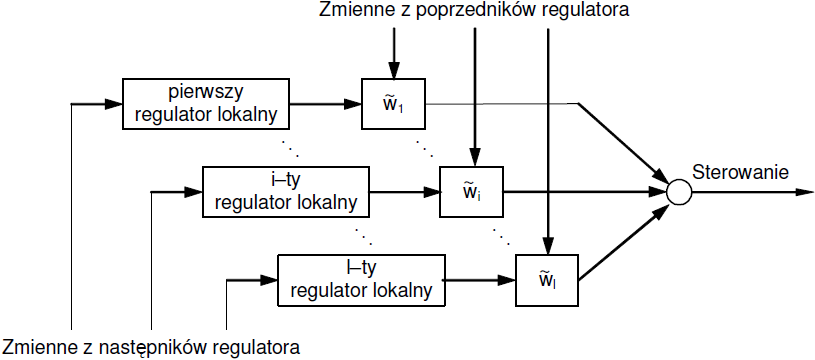
\includegraphics[width=0.75\textwidth]{pictures/pdc}
\caption{Struktura regulatora rozmytego otrzymanego podejściem PDC \cite{171}.}
\label{pdc}
\end{figure}